\subsubsection{Adapted SAGAT}
\label{subsubsec:results_adapted_sagat_2}

The Table \ref{tab:sagat_table_noBase} presents the SAGAT score of all participants on each scene and their average are plotted in the Figures from \ref{fig:barplot_sagat_avg_4_scene_blind} to \ref{fig:barplot_sagat_avg_4_scene}. 


\begin{table}[!htb]
\centering
\caption{SAGAT global score felled by the participants.}
\label{tab:sagat_table_noBase}
\begin{tabular}{lllrrrrr}
\toprule
    &       &        &  Audio & \begin{tabular}[c]{@{}l@{}}Haptic\\ Belt\end{tabular} & \begin{tabular}[c]{@{}l@{}}Virtual\\ Cane\end{tabular} & Mixture \\
Participant & \begin{tabular}[c]{@{}l@{}}Visual\\ Condition\end{tabular} & Round &        &                                                       &                                                        &         \\
\midrule
001C & Blind & First &  5.500 &                                                 5.330 &                                                  5.830 &   3.500 \\
    &       & Return &  6.500 &                                                 8.500 &                                                  5.500 &   5.500 \\
002C & Blind & First &  4.500 &                                                 3.990 &                                                  4.500 &   6.250 \\
    &       & Return &  5.000 &                                                 4.000 &                                                  6.500 &   8.500 \\
003C & Blind & First &  7.500 &                                                 7.490 &                                                  4.660 &   9.000 \\
    &       & Return & 10.000 &                                                 8.500 &                                                  9.000 &   9.000 \\
004C & Blind & First &  6.000 &                                                 7.660 &                                                  4.990 &   6.500 \\
    &       & Return &  6.000 &                                                 9.250 &                                                  7.250 &   9.000 \\
001 & Sight & First &  4.500 &                                                 4.330 &                                                  2.660 &   6.500 \\
    &       & Return &  6.000 &                                                 5.000 &                                                  5.000 &   4.500 \\
003 & Sight & First &  6.750 &                                                 5.990 &                                                  3.990 &   6.750 \\
    &       & Return &  6.000 &                                                 7.250 &                                                  6.250 &   7.500 \\
004 & Sight & First &  7.250 &                                                 7.990 &                                                  5.990 &   8.250 \\
    &       & Return &  7.750 &                                                 9.500 &                                                  8.250 &   7.000 \\
005 & Sight & First &  3.000 &                                                 3.160 &                                                  3.990 &   4.000 \\
    &       & Return &  3.750 &                                                 3.000 &                                                  2.000 &   6.000 \\
\bottomrule
\end{tabular}
\end{table}



The Figures \ref{fig:barplot_sagat_avg_4_scene_blind} and \ref{fig:barplot_sagat_avg_4_scene_sight} also show a increase of the score on in all methods between the rounds for both groups, with only the exception of the "Mixture" method with the sighted users, and the Figure \ref{fig:barplot_sagat_avg_4_scene} shows that the average the blind users were higher than the sighted users.

\begin{figure}[!htb]
    \centering
    \begin{minipage}{\textwidth}
        \centering
        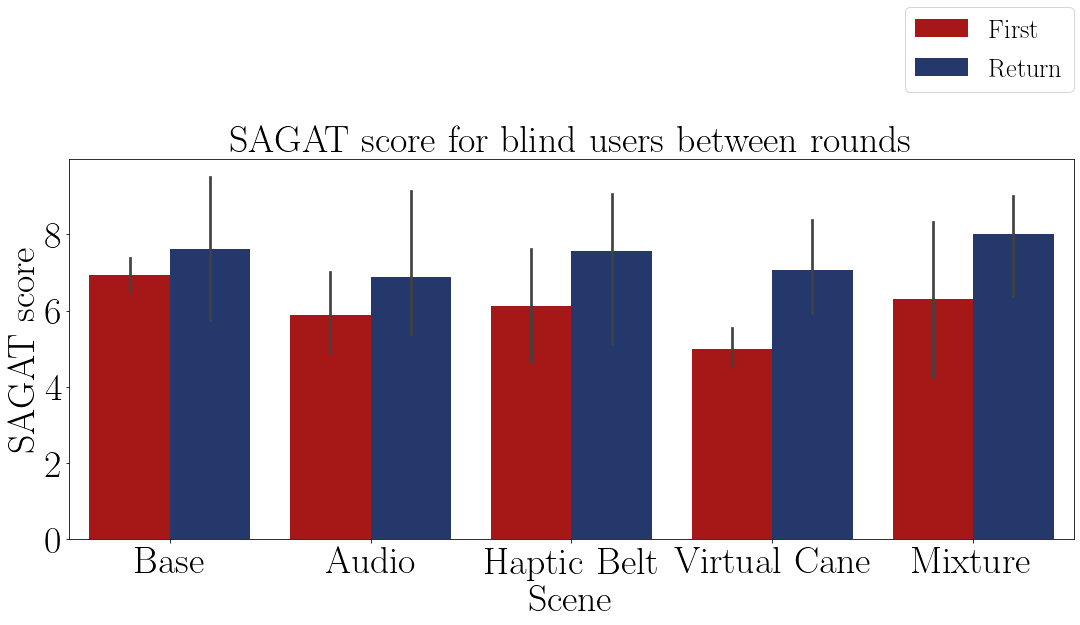
\includegraphics[width = 0.8\linewidth]{Resultados/Sagat/Figuras/png/barplot_sagat_avg_4_scene_blind.png}
        \caption{Barplot of the SAGAT score of the blind participants on each method and round.}
        \label{fig:barplot_sagat_avg_4_scene_blind}
    \end{minipage}
    \begin{minipage}{\textwidth}
        \centering
        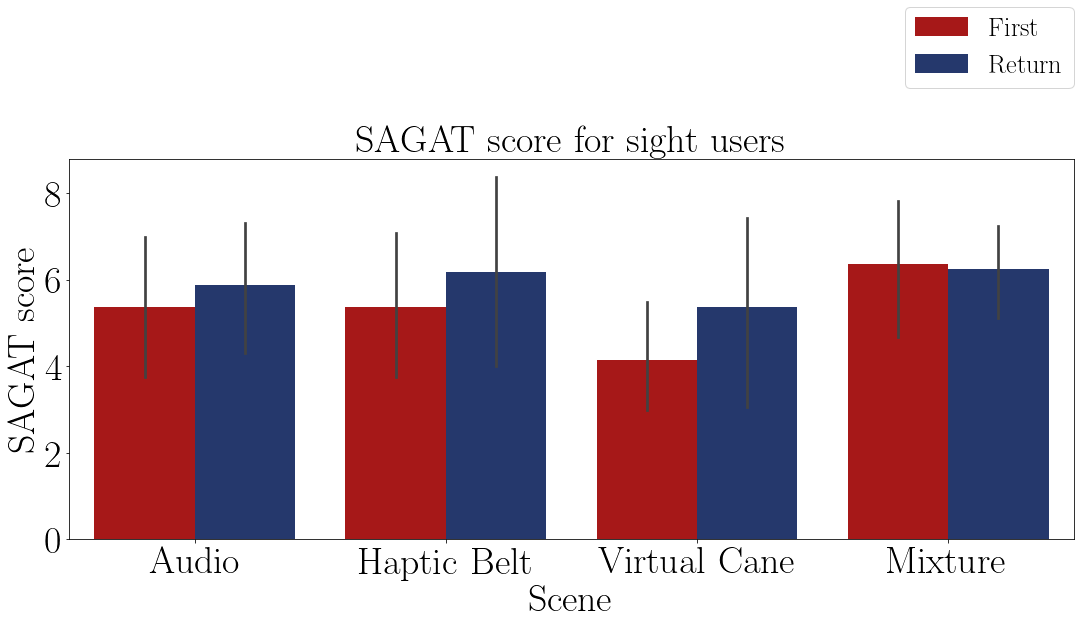
\includegraphics[width = 0.8\linewidth]{Resultados/Sagat/Figuras/png/barplot_sagat_avg_4_scene_sight.png}
        \caption{Barplot of the SAGAT score of the sight participants on each method and round.}
        \label{fig:barplot_sagat_avg_4_scene_sight}
    \end{minipage}
\end{figure}
\begin{figure}[!htb]
    \centering
    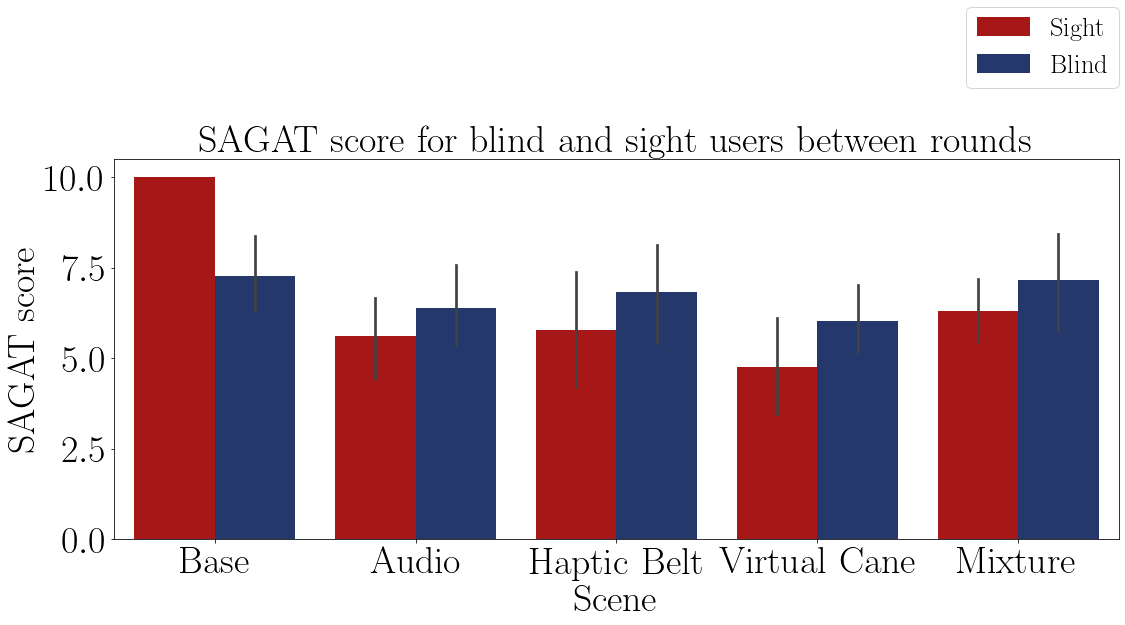
\includegraphics[width = 0.8\linewidth]{Resultados/Sagat/Figuras/png/barplot_sagat_avg_4_scene.png}
    \caption{Barplot of the SAGAT score of both participants on each method.}
    \label{fig:barplot_sagat_avg_4_scene}
\end{figure}

The Figure \ref{fig:boxplot_sagat_4_scene} and \ref{fig:boxplot_sagat_4_rounds} presents a box plot with the SAGAT score of both groups by method and rounds in that order. These figures show that the reaction of each group is also different between the methods and rounds, with the "blind".

\begin{figure}[!htb]
    \centering
    \begin{minipage}{0.45\textwidth}
        \centering
        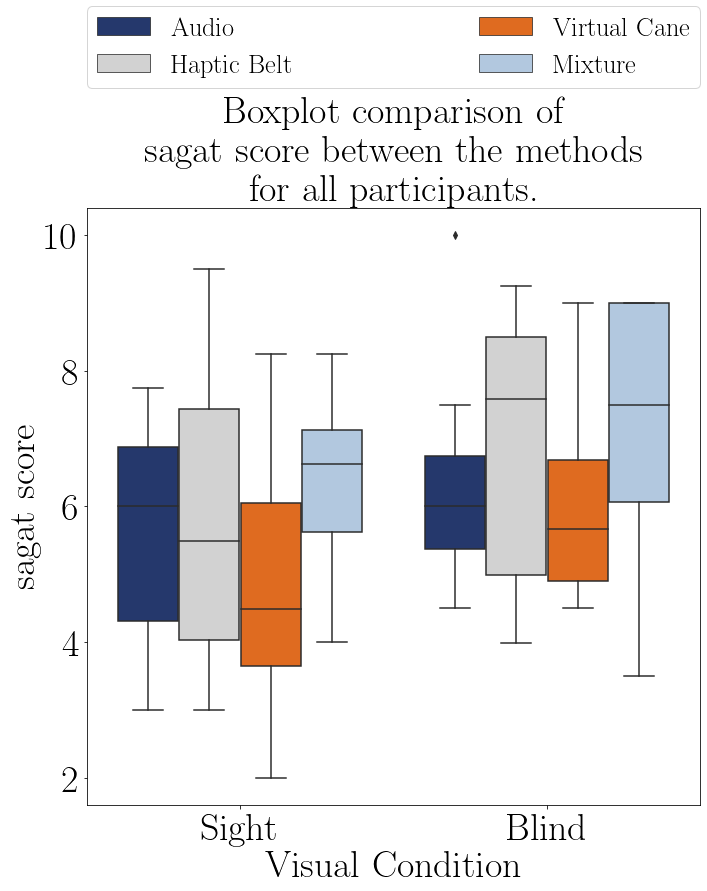
\includegraphics[width = 0.8\linewidth]{Resultados/Sagat/Figuras/png/boxplot_sagat_4_scene.png}
        \caption{Boxplot of the NASA-TLX score of the participants grouped by method.}
        \label{fig:boxplot_sagat_4_scene}
    \end{minipage}
    \begin{minipage}{0.45\textwidth}
        \centering
        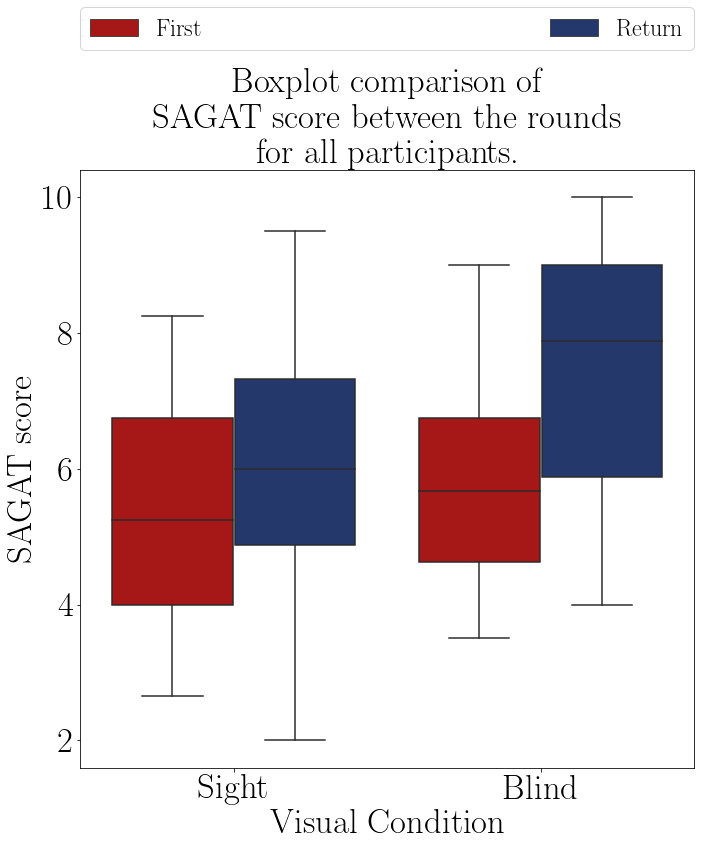
\includegraphics[width = 0.8\linewidth]{Resultados/Sagat/Figuras/png/boxplot_sagat_4_rounds.png}
        \caption{Boxplot of the NASA-TLX score of the participants grouped by round.}
        \label{fig:boxplot_sagat_4_rounds}
    \end{minipage}
\end{figure}

The Table \ref{tab:sagat_average_group_noBase} shows the average SAGAT score of both samples and is possible to notice how the average score by the blind users was higher in every method.


\begin{table}[!htb]
\centering
\caption{Adapted Sagat average global score grouped by participant and visual Condition.}
\label{tab:sagat_average_group_noBase}
\begin{tabular}{lrrrrrr}
\toprule
{} & Audio & \begin{tabular}[c]{@{}l@{}}Haptic\\ Belt\end{tabular} & \begin{tabular}[c]{@{}l@{}}Virtual\\ Cane\end{tabular} &  Mixture \\
Visual Condition &       &                                                       &                                                        &          \\
\midrule
Blind            &  6.38 &                                                  6.84 &                                                   6.03 &    7.156 \\
Sight            &  5.62 &                                                  5.78 &                                                   4.77 &    6.312 \\
\bottomrule
\end{tabular}
\end{table}



The Figures \ref{fig:qqplot_sagat_avg_two_way_sight} and \ref{fig:residplot_sagat_avg_two_way_sight} shows the distribution and variance of sighted participants in the Table \ref{tab:sagat_table_noBase}. These Figures shows that the data are normally distributed and that the methods have a similar variance.
The Table \ref{tab:blocanova_sagat_avg_two_way_sight} shows the ANOVA test p-values of the SAGAT score of the "sight" sample between the guidance methods and they show that the methods had an effect on the score.


\begin{table}[!htb]
\centering
\caption{Anova p-value for the SAGAT score on each method for sighted users.}
\label{tab:blocanova_sagat_avg_two_way_sight}
\begin{tabular}{lrrrrr}
\toprule
               Source &  Squared sum &  DOF & Squared average &      F & \begin{tabular}[c]{@{}l@{}}P-Value \\ $(F_{0} > F)$\end{tabular} \\
\midrule
Participants (Blocks) &       77.492 &    3 &          25.831 & 27.053 &                                                                  \\
         \    Methods &        9.866 &    3 &           3.289 &  3.444 &                                                          0.035** \\
          \    Rounds &        2.910 &    1 &           2.910 &  3.048 &                                                            0.095 \\
     \    Interaction &        1.931 &    3 &           0.644 &  0.674 &                                                            0.578 \\
   Experimental Error &       20.051 &   21 &           0.955 &        &                                                                  \\
                Total &      112.250 &   31 &                 &        &                                                                  \\
\bottomrule
\end{tabular}
\end{table}



\begin{figure}[!htb]
    \centering
    \begin{minipage}{0.45\textwidth}
        \centering
        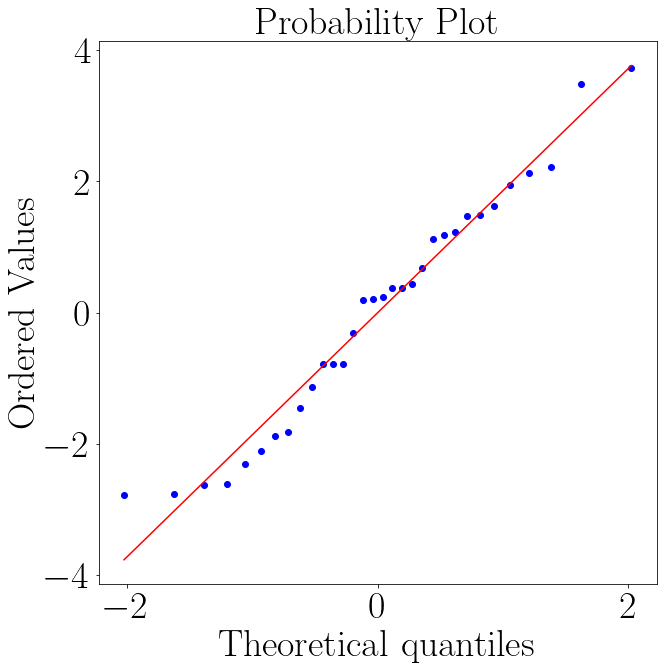
\includegraphics[width = 0.8\linewidth]{Resultados/Sagat/Figuras/png/qqplot_sagat_avg_two_way_sight.png}
        \caption{QQ plot of the mental demand of the sight participants on each method.}
        \label{fig:qqplot_sagat_avg_two_way_sight}
    \end{minipage}
    \begin{minipage}{0.45\textwidth}
        \centering
        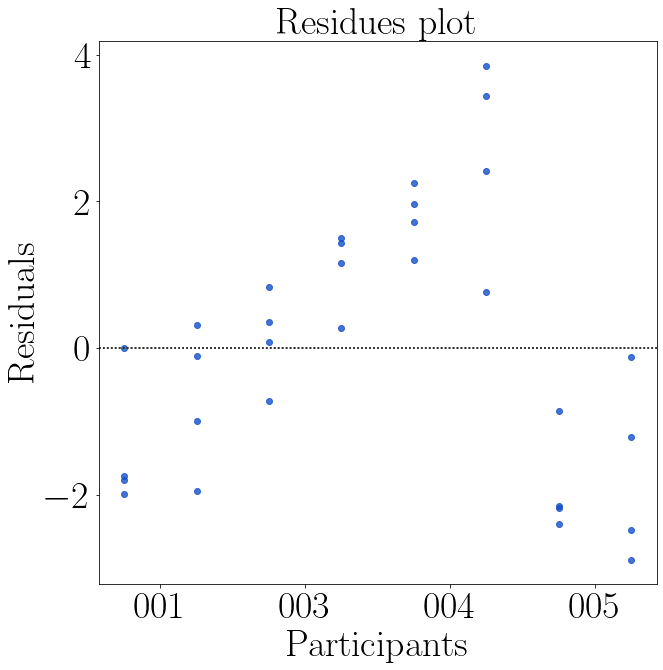
\includegraphics[width = 0.8\linewidth]{Resultados/Sagat/Figuras/png/residplot_sagat_avg_two_way_sight.png}
        \caption{Residual plot of the mental demand score the sight participants on each method.}
        \label{fig:residplot_sagat_avg_two_way_sight}
    \end{minipage}
\end{figure}

The Table \ref{tab:lsd_sagat_avg_two_way_sight} presents the conclusion of a pairwise Fisher LSD test of the previous ANOVA test. The results show that only the "Audio" and the "Haptic Belt" had a similar SAGAT score. This is different than the result from the ANOVA of the blind users, which indicated for them that the rounds had an effect.


\begin{table}[!htb]
\centering
\caption{Cross validation p-value for the SAGAT score on each method for sighted users.}
\label{tab:lsd_sagat_avg_two_way_sight}
\begin{tabular}{rclr}
\toprule
      \multicolumn{3}{c}{Method} &                                           Analysis \\
\midrule
       Audio & $X$ & Haptic Belt &            $H_0 : \mu_{Audio} = \mu_{Haptic Belt}$ \\
      Audio & $X$ & Virtual Cane &       $H_1 : \mu_{Audio} \ne \mu_{Virtual Cane}**$ \\
           Audio & $X$ & Mixture &            $H_1 : \mu_{Audio} \ne \mu_{Mixture}**$ \\
Haptic Belt & $X$ & Virtual Cane & $H_1 : \mu_{Haptic Belt} \ne \mu_{Virtual Cane}**$ \\
     Haptic Belt & $X$ & Mixture &      $H_1 : \mu_{Haptic Belt} \ne \mu_{Mixture}**$ \\
    Virtual Cane & $X$ & Mixture &     $H_1 : \mu_{Virtual Cane} \ne \mu_{Mixture}**$ \\
\bottomrule
\end{tabular}
\end{table}



The Table \ref{tab:sagat_var_group_noBase} shows the average of the SAGAT score variation between the rounds. This table and the Figure \ref{fig:boxplot_sagat_4_rounds} show that, besides the higher average score, the blind users also had a higher variation between the rounds.


\begin{table}[!htb]
\centering
\caption{Adapted Sagat global score variation grouped by participant and visual Condition}
\label{tab:sagat_var_group_noBase}
\begin{tabular}{lrrrrrr}
\toprule
{} &  Audio & \begin{tabular}[c]{@{}l@{}}Haptic\\ Belt\end{tabular} & \begin{tabular}[c]{@{}l@{}}Virtual\\ Cane\end{tabular} & Mixture \\
Visual Condition &        &                                                       &                                                        &         \\
\midrule
Blind            &  15.66 &                                                 23.49 &                                                  44.30 &   32.90 \\
Sight            &  13.53 &                                                 12.59 &                                                  33.12 &    3.80 \\
\bottomrule
\end{tabular}
\end{table}



The Figures \ref{fig:qqplot_sagat_var_sight} and \ref{fig:residplot_sagat_var_sight} shows the distribution and variance of the mental demand variation of the Table \ref{tab:sagat_table_blind}. These Figures shows that the data are normally distributed and that the methods have a similar variance.
The Table \ref{tab:blocanova_sagat_var_sight} shows the Anova test p-value of the SAGAT score of the "sight" sample between the guidance methods and it proves that there is no influence of the methods in the variation of mental demand between the rounds. 


\begin{table}[!htb]
\centering
\caption{Anova p-value for the SAGAT score variation on each method for blinded users.}
\label{tab:blocanova_sagat_var_sight}
\begin{tabular}{lrrrrr}
\toprule
Source & P-Value \\
\midrule
Method &   0.775 \\
\bottomrule
\end{tabular}
\end{table}



\begin{figure}[!htb]
    \centering
    \begin{minipage}{0.45\textwidth}
        \centering
        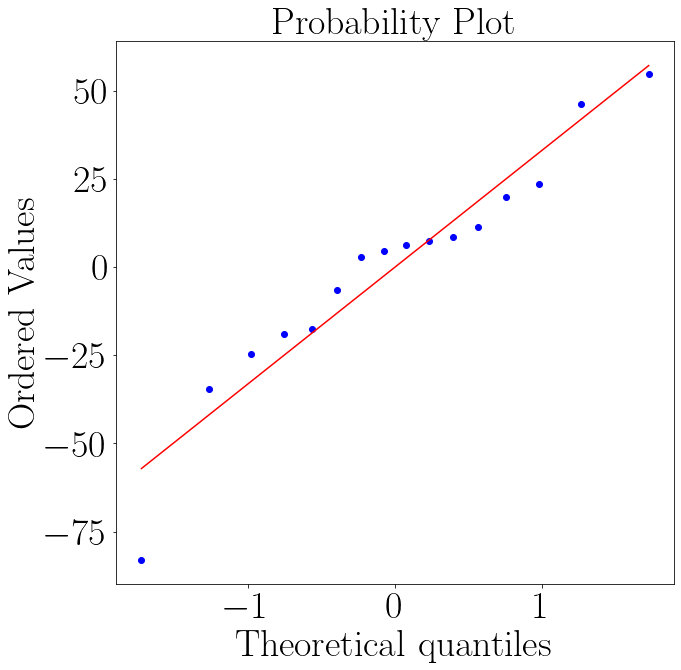
\includegraphics[width = 0.8\linewidth]{Resultados/Sagat/Figuras/png/qqplot_sagat_var_sight.png}
        \caption{Residual plot of the variation SAGAT score of the blind participants on each method.}
        \label{fig:qqplot_sagat_var_sight}
    \end{minipage}
    \begin{minipage}{0.45\textwidth}
        \centering
        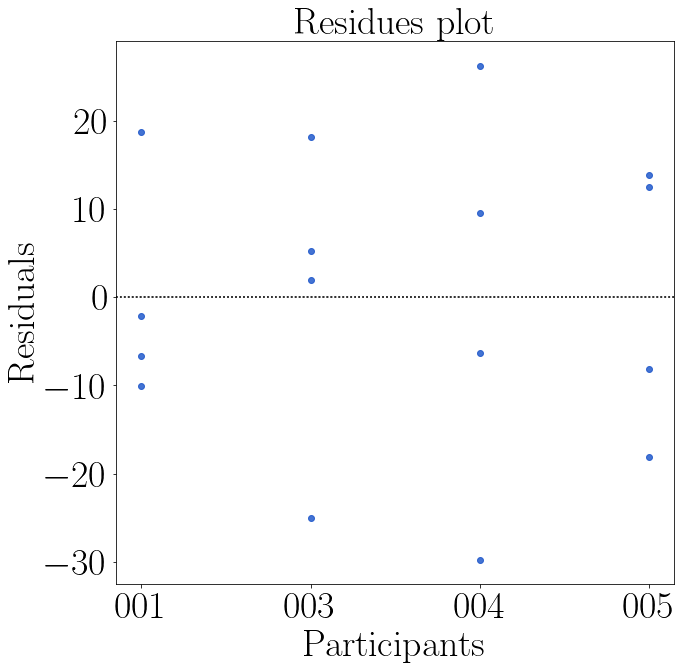
\includegraphics[width = 0.8\linewidth]{Resultados/Sagat/Figuras/png/residplot_sagat_var_sight.png}
        \caption{Residual plot of the variation SAGAT score of the sighted participants on each method.}
        \label{fig:residplot_sagat_var_sight}
    \end{minipage}
\end{figure}

%The Table \ref{tab:lsdbloc_mental_demand_var} presents the conclusion of a pairwise Fisher LSD test of the blind mental demand between all the guidance methods. The results show that all methods have similar variations.

%
\begin{table}[!htb]
\centering
\caption{Cross validation p-value for the mental demand variation on each method for blinded users.}
\label{tab:lsdbloc_mental_demand_var}
\begin{tabular}{rclr}
\toprule
      \multicolumn{3}{c}{Method} &                                       Analysis \\
\midrule
              Base & $X$ & Audio &           $H_1 : \mu_{Base} \ne \mu_{Audio}**$ \\
        Base & $X$ & Haptic Belt &         $H_0 : \mu_{Base} = \mu_{Haptic Belt}$ \\
       Base & $X$ & Virtual Cane &    $H_1 : \mu_{Base} \ne \mu_{Virtual Cane}**$ \\
            Base & $X$ & Mixture &         $H_1 : \mu_{Base} \ne \mu_{Mixture}**$ \\
       Audio & $X$ & Haptic Belt &    $H_1 : \mu_{Audio} \ne \mu_{Haptic Belt}**$ \\
      Audio & $X$ & Virtual Cane &       $H_0 : \mu_{Audio} = \mu_{Virtual Cane}$ \\
           Audio & $X$ & Mixture &            $H_0 : \mu_{Audio} = \mu_{Mixture}$ \\
Haptic Belt & $X$ & Virtual Cane & $H_0 : \mu_{Haptic Belt} = \mu_{Virtual Cane}$ \\
     Haptic Belt & $X$ & Mixture &  $H_1 : \mu_{Haptic Belt} \ne \mu_{Mixture}**$ \\
    Virtual Cane & $X$ & Mixture &     $H_0 : \mu_{Virtual Cane} = \mu_{Mixture}$ \\
\bottomrule
\end{tabular}
\end{table}



To close up, according to the Tables \ref{tab:sagat_average_group_noBase} and \ref{tab:sagat_var_group_noBase} with the Figures \ref{fig:boxplot_sagat_4_scene} and \ref{fig:boxplot_sagat_4_rounds} the blind user scored a higher SAGAT score than the sight user with the same conditions and devices. Besides that, the ANOVA and the LSD Fisher Test at Tables \ref{tab:blocanova_sagat_avg_two_way_sight} and \ref{tab:lsd_sagat_avg_two_way_sight} show that for the sight user the methods impact more their score, whilst the blind user were affected more with the rounds.

There is no influence in the tested methods in the participants mental demand variation, as shown in the Table \ref{tab:blocanova_sagat_var_sight}.

\FloatBarrier